% =====================================================================
% Capítulo 2 (continuación): Secs. 2.7-2.8
%   Pruebas de hipótesis para tablas de conteo y SigTree
% =====================================================================

% ---------------------------------------------------------------------
\section{Pruebas de hipótesis para tablas de conteo}\label{sec:pruebas}

La Sección~\ref{sec:idiv-poisson} mostró que la interacción que queda dentro de un
bloque se mide con el estadístico $G^2$ de una prueba de independencia. Para usar
ese estadístico como criterio de refinamiento hay que resolver tres cuestiones. La
primera es cómo obtener una distribución de referencia válida cuando las tablas
son pequeñas o escasas, cuando los conteos varían entre días más de lo que
admite el modelo de Poisson y cuando los bloques se eligieron con los mismos
datos. La
segunda es cómo controlar el error al realizar muchas pruebas, una por cada bloque
de un árbol de refinamientos. La tercera es cómo evitar que, con millones de
viajes, cualquier diferencia mínima resulte significativa. Esta sección presenta
las herramientas estadísticas que responden a cada una, según resume la
Tabla~\ref{tab:pruebas-mapa}.

\begin{table}[ht]
  \centering
  {\footnotesize
  \renewcommand{\arraystretch}{1.4}
  \begin{tabular}{@{}>{\raggedright\arraybackslash}p{0.56\textwidth}
                  >{\raggedright\arraybackslash}p{0.34\textwidth}@{}}
    \toprule
    \textbf{Cuestión} & \textbf{Subsecciones} \\
    \midrule
    Distribución de referencia válida (tablas pequeñas, sobredispersión,
      grupos elegidos con los mismos datos) &
      \ref{sec:est-independencia}, \ref{sec:est-permutacion},
      \ref{sec:est-bootstrap} y \ref{sec:est-seleccion} \\
    \midrule
    Control del error con muchas pruebas &
      \ref{sec:est-multiplicidad} \\
    \midrule
    Diferencias mínimas significativas con muestras enormes &
      \ref{sec:est-efecto} \\
    \bottomrule
  \end{tabular}
  }
  \caption{Cuestiones que resuelve cada subsección.}
  \label{tab:pruebas-mapa}
\end{table}

A lo largo de la sección se considera una tabla de contingencia genérica
$x = (x_{ij})$ de $a$ filas y $b$ columnas, con totales $x_{i+}$, $x_{+j}$ y
$x_{++}$. En la propuesta, esa tabla será la restricción de la matriz de
co-ocurrencia a un bloque, de modo que $a$ y $b$ serán el número de regiones y de
intervalos que contiene cada bloque. Se usa esta notación genérica, distinta de la
de las secciones anteriores, para subrayar que las herramientas que se presentan
son válidas para cualquier tabla de conteos y no dependen del contexto
espacio-temporal en que se aplicarán.

\subsection{Pruebas de independencia}\label{sec:est-independencia}

La hipótesis nula de independencia afirma que la probabilidad de cada celda es el
producto de las probabilidades marginales, $\pi_{ij} = \pi_{i+}\,\pi_{+j}$, o, en
el modelo de Poisson, que las medias se factorizan como $\mu_{ij} = \alpha_i
\beta_j$. En cualquiera de los dos casos, los conteos esperados estimados bajo la
hipótesis nula son
\begin{equation}\label{eq:esperados}
  \hat{E}_{ij} = \frac{x_{i+}\, x_{+j}}{x_{++}} .
\end{equation}
Las dos pruebas clásicas comparan los conteos observados con estos esperados
\cite{Agresti2013}. La prueba de Pearson usa el estadístico
\begin{equation}\label{eq:pearson}
  X^2 = \sum_{i,j} \frac{(x_{ij} - \hat{E}_{ij})^2}{\hat{E}_{ij}} ,
\end{equation}
y la prueba de razón de verosimilitud usa
\begin{equation}\label{eq:g2}
  G^2 = 2 \sum_{i,j} x_{ij} \log \frac{x_{ij}}{\hat{E}_{ij}} .
\end{equation}
Bajo la hipótesis nula, y cuando los conteos esperados son grandes, ambos
estadísticos siguen aproximadamente una distribución $\chi^2$ con
$(a-1)(b-1)$ grados de libertad, y son asintóticamente equivalentes
\cite{Agresti2013}. Con conteos esperados pequeños la aproximación se deteriora;
la regla práctica más difundida pide que la mayoría de los conteos esperados sean
al menos cinco. Por ejemplo, en la tabla
$\begin{pmatrix} 6 & 2 \\ 2 & 6 \end{pmatrix}$ todos los esperados valen $4$, por
debajo de cinco; los estadísticos valen $X^2 = 4$ y $G^2 = 4.19$, parecidos como
se espera, pero la aproximación $\chi^2$ no es fiable en esta tabla.

El estadístico $G^2$ tiene dos propiedades que lo hacen preferible en esta tesis.
La primera es su conexión con el marco de Bregman, pues como los esperados
\eqref{eq:esperados} reproducen el total de la tabla, los términos lineales de la
I-divergencia se cancelan y $G^2 = 2\,D_I(x \,\|\, \hat{E})$. Por la
ecuación~\eqref{eq:g2-im}, esto equivale a $G^2 = 2\,x_{++}\,\hat{I}(R;T)$, de modo
que el estadístico es la información mutua de la tabla escalada por su masa. La
segunda es que $G^2$ admite una partición exacta, ya que cuando las filas de una tabla se
agrupan, el $G^2$ de la tabla completa es igual al $G^2$ de la tabla colapsada más
la suma de los $G^2$ de las subtablas de cada grupo \cite{Agresti2013}. El
estadístico de Pearson no cumple esta identidad de forma exacta. Esta propiedad
es la que permite, en el Capítulo~\ref{chap:propuesta}, repartir la interacción
de un bloque entre la parte que explica un corte y la que queda dentro de los
hijos. Un ejemplo lo ilustra. La tabla con filas $(8,2)$, $(8,2)$ y $(2,8)$ tiene
$G^2 = 10.36$. Si se agrupan las dos primeras filas, idénticas, la tabla colapsada
$\begin{pmatrix} 16 & 4 \\ 2 & 8 \end{pmatrix}$ tiene $G^2 = 10.36$, y dentro de
cada grupo el $G^2$ es cero, de modo que toda la asociación se explica con ese
corte y no queda nada dentro de los hijos.

\subsection{Pruebas condicionales y p-valores por simulación}\label{sec:est-permutacion}

La distribución $\chi^2$ es solo una aproximación. Para tablas con celdas
escasas, que son frecuentes en bloques de poca actividad, conviene una prueba cuya
validez no dependa del tamaño de la muestra. La idea es eliminar los parámetros
desconocidos condicionando sobre sus estadísticos suficientes, es decir, los resúmenes de los datos que contienen toda la información sobre un parámetro. Bajo la hipótesis
nula de independencia, tanto en el modelo de Poisson como en el multinomial, la
distribución de la tabla condicionada a sus totales de fila y de columna es la
hipergeométrica multivariada, es decir, la forma de repartir los conteos al azar
manteniendo esos totales, que no depende de los parámetros $\alpha_i$ y
$\beta_j$ \cite{Agresti2013}. El p-valor exacto es la probabilidad, bajo esa
distribución, de obtener un estadístico al menos tan extremo como el observado.
Para tablas $2 \times 2$ esta es la prueba exacta de Fisher. En la tabla
$\begin{pmatrix} 6 & 2 \\ 2 & 6 \end{pmatrix}$, con todos los totales iguales a
$8$, las tablas tan extremas como la observada son las que tienen $0$, $1$, $2$,
$6$, $7$ u $8$ en la primera celda, y su probabilidad conjunta es
$1698/12\,870 \approx 0.13$. La aproximación $\chi^2$ daba $p \approx 0.04$, de
modo que sugería evidencia donde la prueba exacta no la encuentra al 5\,\%.

Enumerar todas las tablas con los mismos totales es inviable salvo en tablas muy
pequeñas, por lo que el p-valor se estima por simulación. El algoritmo de
\cite{Patefield1981} genera tablas aleatorias con totales de fila y columna
fijos, con probabilidad igual a la hipergeométrica multivariada. Con $B$ tablas
simuladas y sus estadísticos $t_1, \dots, t_B$, el p-valor se estima como
\begin{equation}\label{eq:pval-mc}
  \hat{p} = \frac{1 + \#\{k : t_k \ge t_{\mathrm{obs}}\}}{1 + B} .
\end{equation}
\cite{Phipson2010} muestran que sumar uno en el numerador y en el denominador no
es un ajuste arbitrario, pues la tabla observada es, bajo la hipótesis nula, una
realización más de la misma distribución, y la fórmula~\eqref{eq:pval-mc} produce
una prueba exacta, mientras que la proporción sin corregir $\#\{k : t_k \ge
t_{\mathrm{obs}}\}/B$ puede valer cero y subestima el p-valor. Una consecuencia
práctica es que el menor p-valor alcanzable es $1/(B+1)$, así que para probar a un
nivel $\alpha$ se necesita $B \ge 1/\alpha - 1$ como mínimo, es decir, $B \ge 19$ para
$\alpha = 0.05$ y $B \ge 99$ para $\alpha = 0.01$. Por ejemplo, con $B = 99$ y
cuatro tablas simuladas por encima de la observada, $\hat{p} = (1+4)/100 = 0.05$.

Cuando se realizan muchas pruebas, la mayoría con p-valores grandes, simular $B$
tablas en todas ellas desperdicia cómputo. \cite{Besag1991} propusieron un
procedimiento secuencial en el que se simulan tablas hasta que $h$ de ellas superan al
estadístico observado, o hasta alcanzar un máximo $B$. Si la simulación se detiene
tras $l$ tablas, el p-valor es $h/l$; si no, se usa la fórmula anterior. El
procedimiento mantiene la validez de la prueba y detiene pronto la simulación en
los casos claramente no significativos.

Un aspecto de las pruebas por simulación que se usará después es que el
estadístico puede ser cualquier función de la tabla, incluida una que involucre
una búsqueda. Si $t$ es, por ejemplo, el máximo de $G^2$ sobre un conjunto de
divisiones candidatas, el p-valor~\eqref{eq:pval-mc} sigue siendo válido siempre
que en cada tabla simulada se repita la misma búsqueda. Esta es la base del ajuste
por selección de la Sección~\ref{sec:est-seleccion}.

\subsection{Remuestreo de réplicas independientes}\label{sec:est-bootstrap}

La prueba condicional anterior es exacta solo si los conteos son de Poisson.
Cuando no lo son, la distribución de referencia debe reflejar la variabilidad
real de los datos, y una forma de obtenerla sin suponer un modelo es el
\emph{bootstrap} \cite{Efron1993}. Si la tabla observada es la suma de $D$
réplicas independientes y con la misma distribución, $x = \sum_{d=1}^{D} x_d$,
la distribución de un estadístico de $x$ se aproxima remuestreando $D$ réplicas
con reemplazo entre las observadas y recalculando el estadístico sobre su suma.
Por ejemplo, con $12$ días laborables, cada réplica del \emph{bootstrap} elige $12$
días al azar con reemplazo, de modo que algunos se repiten y otros no aparecen, y
suma sus matrices diarias.

Para una prueba de hipótesis, el remuestreo debe hacerse bajo la hipótesis
nula, aunque los datos observados no la cumplan; de lo contrario, la
distribución de referencia incluiría el propio efecto que se quiere detectar y
la prueba perdería potencia \cite{HallWilson1991}. La forma habitual es
desplazar o reescalar las réplicas para que su media sea la estimada bajo la
hipótesis nula, de modo que el remuestreo conserve la variabilidad de los datos
pero no su desviación respecto del nulo.

Con pocas réplicas conviene una corrección adicional. La varianza empírica de
$D$ réplicas subestima la poblacional en un factor $(D-1)/D$, de modo que las
desviaciones de cada réplica respecto de su media se multiplican por
$\sqrt{D/(D-1)}$ antes de remuestrear. El supuesto que no se puede eludir es la
independencia entre réplicas, ya que si las réplicas están correlacionadas, como dos
días consecutivos con el mismo episodio de clima, el remuestreo subestima la
variabilidad.

\subsection{Comparaciones múltiples}\label{sec:est-multiplicidad}

Cuando se realizan $M$ pruebas, cada una a un nivel $\alpha$, la probabilidad de
cometer al menos un falso rechazo crece con $M$. Con $\alpha = 0.05$ esa probabilidad es $1-(1-\alpha)^M$, que vale $0.05$ con una prueba, $0.64$ con $20$ y $0.99$ con $100$. Dos medidas de error resumen el
problema. La tasa de error por familia (FWER) es la probabilidad de cometer al
menos un falso rechazo. La tasa de falsos descubrimientos (FDR) es la proporción
esperada de falsos rechazos entre todos los rechazos \cite{Benjamini1995}.
Controlar la FWER es más estricto; controlar la FDR tolera algunos falsos
rechazos a cambio de más potencia, lo que suele ser preferible en análisis
exploratorios con muchas hipótesis.

La corrección de Bonferroni prueba cada hipótesis al nivel $\alpha/M$ y controla la
FWER sin ningún supuesto sobre la dependencia entre pruebas. Su costo es la
potencia, ya que cuando las pruebas están correlacionadas, como ocurre al evaluar
divisiones candidatas de un mismo bloque, que comparten casi todos sus datos, la
corrección es mucho más conservadora de lo necesario. El ajuste \emph{min-P} de
\cite{Westfall1993} resuelve este problema usando remuestreo, pues en lugar de dividir
$\alpha$ entre $M$, compara el menor p-valor observado, o de forma equivalente el
mayor estadístico, con su distribución bajo la hipótesis nula conjunta, obtenida
por simulación. Así el ajuste tiene en cuenta a la vez el número de pruebas y la
correlación entre ellas. \cite{Benjamini1995} propusieron, para la FDR, un
procedimiento secuencial sobre los p-valores ordenados que controla esa tasa
cuando las pruebas son independientes.

\paragraph{Pruebas jerárquicas.} En muchos problemas las hipótesis forman un
árbol, y la hipótesis de un nodo solo tiene sentido si la de su padre fue
rechazada. En ese caso no es necesario corregir por todas las pruebas posibles,
sino solo por las que efectivamente se realizan. \cite{Meinshausen2008} propuso un
procedimiento de arriba abajo para grupos jerárquicos de variables, en el que el
nivel asignado a cada grupo es proporcional a su tamaño, y mostró que controla la FWER sobre toda la jerarquía. Por ejemplo, un grupo con el 60\,\% de las variables de su padre recibe el 60\,\% del nivel de este. \cite{Kimes2017} aplicaron una idea análoga al
agrupamiento jerárquico, ya que recorren el dendrograma desde la raíz, prueban en cada
nodo si la división en dos grupos es significativa mediante una prueba por
simulación, y controlan la FWER asignando a cada nodo un umbral proporcional a su
número de observaciones. Para la FDR, \cite{Yekutieli2008} propuso aplicar el
procedimiento de \cite{Benjamini1995} dentro de cada familia de hijos de una
hipótesis rechazada, y acotó la FDR resultante sobre el árbol completo.

Estos procedimientos aprovechan una estructura que también tiene el problema de
esta tesis. Si la hipótesis nula de independencia se cumple en un bloque, se
cumple en todos sus sub-bloques, porque cualquier subtabla de una tabla con medias
factorizadas también las tiene factorizadas. Por lo tanto, las hipótesis nulas
verdaderas forman subárboles completos, y un falso rechazo solo puede producirse
por primera vez en la raíz de uno de ellos.
 La Figura~\ref{fig:subarboles-nulos} lo ilustra.

\begin{figure}[ht]
  \centering
  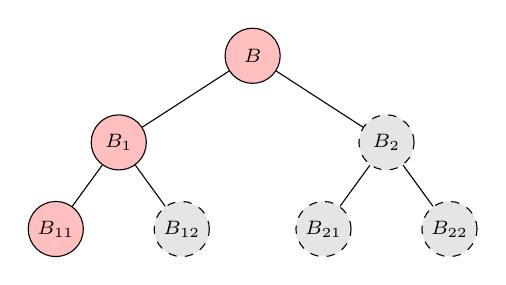
\begin{tikzpicture}[level distance=1.1cm,
      every node/.style={circle, draw, minimum size=0.7cm, inner sep=0pt, font=\scriptsize},
      sibling distance=3.4cm,
      level 2/.style={sibling distance=1.6cm}]
    \node[fill=red!25] {$B$}
      child { node[fill=red!25] {$B_1$}
        child { node[fill=red!25] {$B_{11}$} }
        child { node[fill=gray!20, dashed] {$B_{12}$} } }
      child { node[fill=gray!20, dashed] {$B_2$}
        child { node[fill=gray!20, dashed] {$B_{21}$} }
        child { node[fill=gray!20, dashed] {$B_{22}$} } };
  \end{tikzpicture}
  \caption{Árbol de bloques. En rojo, hipótesis nulas falsas, que se rechazan. En
  gris, hipótesis nulas verdaderas, que son la de $B_2$ y, por tanto, la de todo su subárbol, y la de $B_{12}$. Un falso rechazo solo puede ocurrir por primera vez en $B_2$ o en $B_{12}$, no en sus descendientes.}
  \label{fig:subarboles-nulos}
\end{figure}

\subsection{Inferencia después de la selección}\label{sec:est-seleccion}

Las garantías anteriores suponen que las hipótesis se fijan antes de ver los
datos. En el agrupamiento no ocurre así, ya que los grupos, y por tanto las
hipótesis que se prueban sobre ellos, se eligen con los mismos datos. Este
problema se conoce como doble uso de los datos. \cite{Gao2024} mostraron que, cuando los grupos
se definen mediante agrupamiento, una prueba clásica de diferencia de medias
tiene una tasa de error de tipo~I extremadamente inflada, y que el problema
persiste aunque se usen dos conjuntos de datos independientes para definir los
grupos y para probarlos. La razón es que el procedimiento de agrupamiento
encuentra grupos distintos incluso cuando no hay estructura, y la prueba clásica no lo tiene en cuenta. Por ejemplo, si se generan datos de puro ruido, se agrupan en dos y se prueba si los grupos difieren, la prueba resulta significativa casi siempre. Existen tres
formas de abordar el problema, que la Sección~\ref{sec:ea_inferencia} revisa con
más detalle y que se describen a continuación.

\begin{enumerate}
  \item \textbf{Incluir la selección en la simulación.} Si la prueba es por
  simulación, basta con repetir el procedimiento de selección completo en cada
  réplica nula, como se indicó al final de la Sección~\ref{sec:est-permutacion}.
  El p-valor resultante es válido para la hipótesis nula global de que no hay
  estructura en la tabla, aunque no para hipótesis más específicas.
  \item \textbf{Inferencia selectiva.} Se calcula el p-valor condicionando sobre
  el evento de que el procedimiento haya producido los grupos observados. Es el
  enfoque de \cite{Gao2024} para el agrupamiento jerárquico y de
  \cite{Watanabe2021si} para modelos de bloques latentes. Ofrece garantías
  formales, pero se ha desarrollado sobre todo para datos gaussianos y su costo
  computacional es alto.
  \item \textbf{División de cada observación.} Para conteos de Poisson,
  \cite{Neufeld2024cs} proponen el \emph{count splitting}, en el que cada conteo se divide
  como $x_{ij} = x^{(1)}_{ij} + x^{(2)}_{ij}$, con $x^{(1)}_{ij} \mid x_{ij} \sim
  \mathrm{Binomial}(x_{ij}, \varepsilon)$. Si $x_{ij} \sim
  \mathrm{Poisson}(\mu_{ij})$, las dos partes son independientes y de Poisson, con
  medias $\varepsilon\mu_{ij}$ y $(1-\varepsilon)\mu_{ij}$. Por ejemplo, una celda con $\mu = 10$ y $\varepsilon = 0.5$ produce dos partes independientes con distribución de Poisson de media $5$. La estructura se
  elige con $x^{(1)}$ y se prueba con $x^{(2)}$ como si hubiera sido fijada de
  antemano. \cite{Neufeld2024dt} generalizan la idea, con el nombre de
  \emph{data thinning}, a otras familias de distribuciones cerradas bajo convolución, es decir, aquellas en las que la suma de dos variables sigue en la familia. Si los conteos presentan sobredispersión, las dos partes dejan de
  ser independientes y la garantía se debilita.
\end{enumerate}

\subsection{Tamaño de efecto y sobredispersión}\label{sec:est-efecto}

\paragraph{Tamaño de efecto.} Con muestras grandes, una prueba de hipótesis
detecta desviaciones de la hipótesis nula por pequeñas que sean. En el caso de la
independencia esto se ve directamente, pues por la relación $G^2 = 2\,x_{++}\,\hat
I(R;T)$, si la información mutua de la población es positiva, aunque sea
mínima, el estadístico crece de forma proporcional al número de observaciones y
el p-valor tiende a cero. Con $\hat I = 0.001$ nats, $G^2 = 2$ si $x_{++} = 1\,000$, pero $G^2 = 2\,000$ si $x_{++} = 10^6$. Los propios \cite[Sec.~5]{Hu2025} identifican este
fenómeno como una limitación de SigTree. Con millones de viajes, la
significancia deja de distinguir entre interacciones relevantes e irrelevantes.

La respuesta habitual es acompañar la significancia con una medida de tamaño de
efecto que no crezca con la muestra. Para tablas de contingencia hay dos opciones
naturales. La primera es la propia información mutua por observación,
$\hat I(R;T) = G^2/(2\,x_{++})$, medida en nats, que conecta directamente con la
función objetivo del co-agrupamiento. La segunda es la $V$ de Cramér,
\begin{equation}\label{eq:cramer}
  V = \sqrt{\frac{X^2}{x_{++}\,\min(a-1,\, b-1)}} ,
\end{equation}
que toma valores entre 0, bajo independencia, y 1, bajo asociación perfecta
\cite{Agresti2013}. Ambas permiten fijar un umbral de relevancia independiente
del tamaño de la muestra. Por ejemplo, la tabla $\begin{pmatrix} 6 & 2 \\ 2 & 6 \end{pmatrix}$ tiene $V = 0.5$ e $\hat I = 0.131$ nats; multiplicada por $100$, su $G^2$ pasa de $4.19$ a $419$, pero $V$ e $\hat I$ no cambian.

La información mutua empírica tiene, sin embargo, un sesgo positivo que importa
en tablas pequeñas. Aunque la población sea independiente, $G^2$ sigue
aproximadamente una $\chi^2$ con $\nu = (a-1)(b-1)$ grados de libertad, cuya
media es $\nu$, de modo que $\mathrm{E}[\hat I(R;T)] \approx \nu/(2\,x_{++}) > 0$.
Es el mismo sesgo que describe la corrección de Miller y Madow para los
estimadores de entropía e información mutua \cite{Paninski2003}. Un umbral
sobre $\hat I$ sin corregir favorecería, por tanto, a las tablas con pocas observaciones y muchas celdas, como ocurre con $x_{++} = 100$, donde el sesgo esperado es $0.005$ nats en una tabla $2 \times 2$ y $0.08$ en una $5 \times 5$.

\paragraph{Sobredispersión.} El modelo de Poisson impone que la varianza de cada
conteo sea igual a su media. En datos reales es frecuente que la varianza sea
mayor, $\mathrm{Var}(x_{ij}) = \varphi\,\mu_{ij}$ con $\varphi > 1$, porque los
eventos no son independientes, como ocurre en movilidad, donde la actividad de una celda varía de un
día a otro por el día de la semana, el clima o eventos puntuales. En ese caso los
estadísticos $X^2$ y $G^2$ se inflan aproximadamente por el factor $\varphi$, y
una prueba calibrada bajo el modelo de Poisson rechaza la hipótesis nula con
demasiada frecuencia. El enfoque de cuasi-verosimilitud, que ajusta la varianza sin suponer una distribución completa, corrige este efecto
dividiendo los estadísticos entre una estimación de $\varphi$, por ejemplo el
cociente entre el estadístico de Pearson y sus grados de libertad
\cite{McCullagh1989}. Cuando la matriz se construye agregando varios días, como en
esta tesis, $\varphi$ también puede estimarse a partir de la variación de cada
celda entre días.

Un único $\varphi$ supone que la varianza es proporcional a la media. La
cuasi-verosimilitud admite, más en general, una función de varianza
$\mathrm{Var}(x_{ij}) = V(\mu_{ij})$ \cite{McCullagh1989}. Dos formas habituales
para conteos son la de la binomial negativa, $V(\mu) = \mu + \mu^2/k$, en la que
la sobredispersión aumenta con la media (con $k = 50$, la varianza es $12$ si $\mu = 10$ y $300$ si $\mu = 100$), y la ley de potencia
$V(\mu) = a\,\mu^b$, propuesta por \cite{Taylor1961} para la agregación de
poblaciones biológicas, que contiene como casos particulares la de Poisson
($a=b=1$) y la de $\varphi$ constante ($b=1$).

Todas estas formas describen la varianza de cada celda por separado. Cuando la
variabilidad proviene de factores que actúan sobre muchas celdas a la vez, como
el clima de un día, los conteos de celdas distintas dejan además de ser
independientes, y ningún modelo de varianza por celda describe esa correlación.
Si se dispone de réplicas independientes del periodo, como los días que forman
la matriz, la correlación puede reproducirse por remuestreo
(Sección~\ref{sec:est-bootstrap}) en lugar de modelarse.

% ---------------------------------------------------------------------
\section{Agrupamiento guiado por pruebas de hipótesis con SigTree}\label{sec:sigtree}

Los árboles de decisión son uno de los modelos más usados para producir
agrupamientos interpretables, porque cada grupo queda descrito por la secuencia de
reglas que lleva a su hoja \cite{Hu2025}. En la mayoría de los métodos, sin
embargo, la decisión de dividir un nodo no tiene una interpretación estadística.
La idea de usar pruebas de hipótesis para decidir las divisiones tiene un
antecedente supervisado en CHAID \cite{Kass1980}, que elige las divisiones de un
árbol de clasificación con pruebas $\chi^2$ entre cada división candidata y la
variable de clase. \cite{Hu2025} trasladaron esta idea al caso no supervisado con
SigTree, un algoritmo que construye un árbol de decisión binario para agrupar
datos categóricos y que usa una prueba de hipótesis tanto para elegir cada
división como para decidir cuándo detenerse. Su principal atractivo es que no requiere fijar el número de grupos, lo que atiende una limitación de ST-CC (Sección~\ref{sec:stcc-limitaciones}).

\subsection{Divisiones candidatas y pseudo-clases}

Sea un conjunto de $n$ muestras descritas por $m$ atributos categóricos, donde el
atributo $q$ tiene $k_q$ categorías. En cada nodo, SigTree considera como división
candidata cada categoría $c$ de cada atributo $j$, de modo que la división separa las muestras
que toman el valor $c$ en el atributo $j$ de las que no, y se representa con una
variable binaria $Z = \mathbb{1}[x_j = c]$. Como no hay una variable de clase,
cada uno de los otros $m-1$ atributos actúa como pseudo-clase, es decir, como etiqueta provisional, ya que no hay una variable de clase. La hipótesis
nula de cada prueba es que $Z$ es independiente del atributo $q$, y la hipótesis
nula global es que $Z$ es independiente de todos los demás atributos. La intuición
es que, si las muestras del nodo no tienen estructura de grupos, ninguna división
candidata estará asociada con la mayoría de las pseudo-clases \cite[Sec.~3]{Hu2025}.

\subsection{Estadístico y criterio de división}

Para cada par formado por la división $Z$ y un atributo $q \ne j$ se construye la
tabla de contingencia $2 \times k_q$ de sus frecuencias conjuntas y se calcula el
estadístico de Pearson $X^2(Z, q)$ de la ecuación~\eqref{eq:pearson}. En tablas
$2 \times 2$ con algún conteo esperado menor que cinco se aplica la corrección de Yates, un ajuste que evita sobrestimar el estadístico con conteos pequeños. Los estadísticos de todos los atributos se suman,
\begin{equation}\label{eq:sigtree}
  X^2(Z) = \sum_{q \ne j} X^2(Z, q), \qquad
  \mathrm{gl}(Z) = \sum_{q \ne j} (k_q - 1),
\end{equation}
y el p-valor de la división se obtiene de la distribución $\chi^2$ con
$\mathrm{gl}(Z)$ grados de libertad, bajo el supuesto de que las pruebas
individuales son independientes \cite[Sec.~3.3]{Hu2025}. En cada nodo se elige la
división candidata con menor p-valor. Por ejemplo, en un nodo con $100$ muestras y tres atributos binarios $A$, $B$ y $C$, se prueba la división $Z = \mathbb{1}[A = 1]$, que separa $50$ muestras de otras $50$. Frente a $B$ la tabla es $\begin{pmatrix} 40 & 10 \\ 10 & 40 \end{pmatrix}$, con esperados de $25$ y $X^2 = 36$; frente a $C$ es $\begin{pmatrix} 30 & 20 \\ 20 & 30 \end{pmatrix}$ y $X^2 = 4$. La suma es $X^2(Z) = 40$ con $2$ grados de libertad, y su p-valor es $e^{-20} \approx 2 \cdot 10^{-9}$, lo que indica que la división está muy asociada con $B$ y poco con $C$, y la suma lo recoge.

\subsection{Criterios de parada}

La división elegida solo se aplica si su p-valor es menor o igual que un nivel
ajustado $\alpha^\ast$. Para controlar la FWER al elegir la mejor de muchas
candidatas, SigTree usa la corrección de Bonferroni con un divisor constante,
el número total de categorías de todos los atributos, $|Q|$, de manera que
\begin{equation}\label{eq:sigtree-alpha}
  \alpha^\ast = \frac{\alpha}{|Q|} ,
\end{equation}
que se aplica por igual en todos los nodos \cite[Sec.~3.4]{Hu2025}. En el ejemplo anterior, con tres atributos binarios, $|Q| = 6$ y $\alpha^\ast = 0.05/6 \approx 0.0083$, de modo que la división se acepta. Además, se
usan dos reglas triviales, a saber, no se dividen nodos con cinco muestras o menos, y no se
aceptan divisiones que produzcan un hijo con menos de tres muestras. El
crecimiento termina cuando ninguna hoja admite una división significativa, y las
hojas del árbol son los grupos finales. El resultado es un algoritmo con un solo
parámetro con interpretación estadística clara, el nivel $\alpha$, que no
requiere fijar el número de grupos de antemano.

\subsection{Limitaciones}

Los autores reconocen tres limitaciones \cite[Sec.~5]{Hu2025}. Evaluar todas las
divisiones candidatas en cada nodo es costoso. El algoritmo no optimiza una
función objetivo explícita, por lo que no hay garantía de que el árbol obtenido
sea el mejor posible. Y, como se discutió en la Sección~\ref{sec:est-efecto}, el
estadístico $\chi^2$ crece con el número de muestras y de atributos, lo que empuja
los p-valores hacia cero y dificulta controlar los falsos descubrimientos con el
umbral~\eqref{eq:sigtree-alpha}. A estas se pueden añadir dos observaciones desde
la Sección~\ref{sec:pruebas}. La primera es que el p-valor de la división elegida
se calcula como si esa división se hubiera fijado de antemano, sin tener en cuenta
que se eligió por ser la de menor p-valor (Sección~\ref{sec:est-seleccion}). La
segunda es que la suma~\eqref{eq:sigtree} supone independencia entre pruebas que
comparten la misma variable $Z$, lo que no se cumple en general porque todas ellas
dependen de la misma división. Estas dos observaciones muestran que, aunque el
principio de SigTree es sólido, su traslado a otro dominio exige revisar con
cuidado cómo se obtiene la distribución de referencia de cada prueba.

\subsection{Relación con la propuesta}\label{sec:sigtree-propuesta}

La propuesta de esta tesis toma de SigTree su principio central, construir una
partición con pruebas de hipótesis y detenerse cuando ninguna división es
significativa, y lo traslada al refinamiento de los bloques de ST-CC. Esa
traslación exige adaptar cada componente. La Tabla~\ref{tab:sigtree-astcc} resume
la correspondencia, que se desarrolla en el Capítulo~\ref{chap:propuesta}.

\begin{table}[ht]
  \centering
  {\footnotesize
  \begin{tabular}{@{}>{\raggedright\arraybackslash}p{0.2\textwidth}
                  >{\raggedright\arraybackslash}p{0.34\textwidth}
                  >{\raggedright\arraybackslash}p{0.36\textwidth}@{}}
    \toprule
    \textbf{Componente} & \textbf{SigTree} & \textbf{Propuesta} \\
    \midrule
    Objeto que se divide & Conjunto de muestras con atributos categóricos &
      Bloque de una matriz de conteos región~$\times$~tiempo \\
    División candidata & Presencia o ausencia de una categoría &
      Bipartición de las filas, de las columnas o de ambas a la vez \\
    Qué se prueba & Asociación entre la división y los demás atributos &
      Asociación entre la división y la otra dimensión del bloque \\
    Estadístico & Suma de estadísticos $X^2$ & $G^2$ de la tabla colapsada,
      coherente con la I-divergencia \\
    Distribución de referencia & $\chi^2$ asintótica & \emph{Bootstrap} de los días
      alrededor de la independencia del bloque, repitiendo la búsqueda \\
    Comparaciones múltiples & Bonferroni uniforme & Reparto jerárquico del nivel
      a lo largo del árbol \\
    Criterio de parada & Significancia y reglas triviales & Significancia, tamaño
      de efecto corregido por sesgo y reglas triviales \\
    \bottomrule
  \end{tabular}
  }
  \caption{Correspondencia entre SigTree \cite{Hu2025} y el método propuesto.}
  \label{tab:sigtree-astcc}
\end{table}

Cada fila de la tabla se apoya en una herramienta de la Sección~\ref{sec:pruebas}. El $G^2$ se apoya en su partición exacta (Sección~\ref{sec:est-independencia}); la referencia por \emph{bootstrap} de los días, repitiendo la búsqueda, en el remuestreo y en la inferencia después de la selección (Secciones~\ref{sec:est-bootstrap} y~\ref{sec:est-seleccion}); el reparto jerárquico del nivel, en las pruebas jerárquicas (Sección~\ref{sec:est-multiplicidad}); y el tamaño de efecto corregido por sesgo, en la Sección~\ref{sec:est-efecto}. Las limitaciones de los dos métodos base orientan además el diseño. La elección
heurística del número de grupos en ST-CC (Sección~\ref{sec:stcc-limitaciones})
motiva que la resolución final no dependa solo de $K_R$ y $K_T$, y la inflación
del estadístico de SigTree con muestras grandes motiva complementar la
significancia con un umbral de tamaño de efecto.
